\documentclass{article}
\usepackage[left=0.5in,top=0.5in,right=0.5in,bottom=0.5in]{geometry}
\usepackage[english]{babel}
\usepackage[utf8]{inputenc}
\usepackage{graphicx}
\usepackage{amssymb,amsmath,amsthm,latexsym}
\graphicspath{{./images/}}
\begin{document}
% \begin{align*}
%   \text{Linear charge density; }\lambda &= \frac{q}{\mathcal{L}}, \text{where q is the charge and \(\mathcal{L}\) is the length over which it is distributed. The SI unit is}~cm^{-1}\\
%   \text{Surface charge density; } \sigma &= \frac{q}{\mathcal{A}}, \text{where q is the charge and \(\mathcal{A}\) is the area of the surface. The SI unit is}~cm^{-2}\\
%   \text{Volume charge density; } \rho &= \frac{q}{\mathcal{V}}, \text{where q is the charge and \(\mathcal{V}\) is the volume distribution. The SI unit is}~cm^{-3}
% \end{align*}
\begin{enumerate}
  \item[1.] A region of space contains an electric field \( \overrightarrow{E} = E_1 \widehat{i} + E_2 \widehat{j} \) where \(E_1\) and \(E_2\) are positive constants. A frame whose corners are located at (x, y, z) = (\(\frac{a}{2}\), 0, \(\frac{a}{2}\)), (\(\frac{-a}{2}\), 0,\(\frac{-a}{2}\)), (\(\frac{a}{2}\), 0,\(\frac{-a}{2}\)), and (\(\frac{-a}{2}\), 0, \(\frac{a}{2}\)). What is the magnitude of the electric flux through the frame?
  \begin{align*}
    \overrightarrow{E} =&~E_1\widehat{i} + E_2\widehat{j}\\
    A =~(\frac{a}{2},0,\frac{a}{2}),~B =~(-\frac{a}{2},0,-\frac{a}{2}),&~C =~(\frac{a}{2},0,-\frac{a}{2}),~D =~(-\frac{a}{2},0,\frac{a}{2})\\
    \text{Area of rectangle:}&~(L\cdot{W})\widehat{j}\\
    \cdots \\
    \phi_E =&~\overrightarrow{E}\cdot\overrightarrow{A}\\
           =&~(E_1\widehat{i} + E_2\widehat{j})\cdot{a}^2(\pm \widehat{j})\\
           =&~E_1a^2(\widehat{i}\cdot{(\pm\widehat{j})}) + E_2a^2(\widehat{j}\cdot{(\pm{\widehat{j}})})\\
           =&~0+E_2a^2(\pm{1})\\
           =&~\pm E_2a^2\\
           \widehat{i}\widehat{j} &= \widehat{i}(-\widehat{j}) = 0\\
           \widehat{j}\widehat{j} &= 1\cdot\widehat{j}(-\widehat{j}) = -1\\
           |\phi_E|=|\pm E_2a^2|&=\boxed{E_2a^2}
  \end{align*}
  \item[] \begin{center}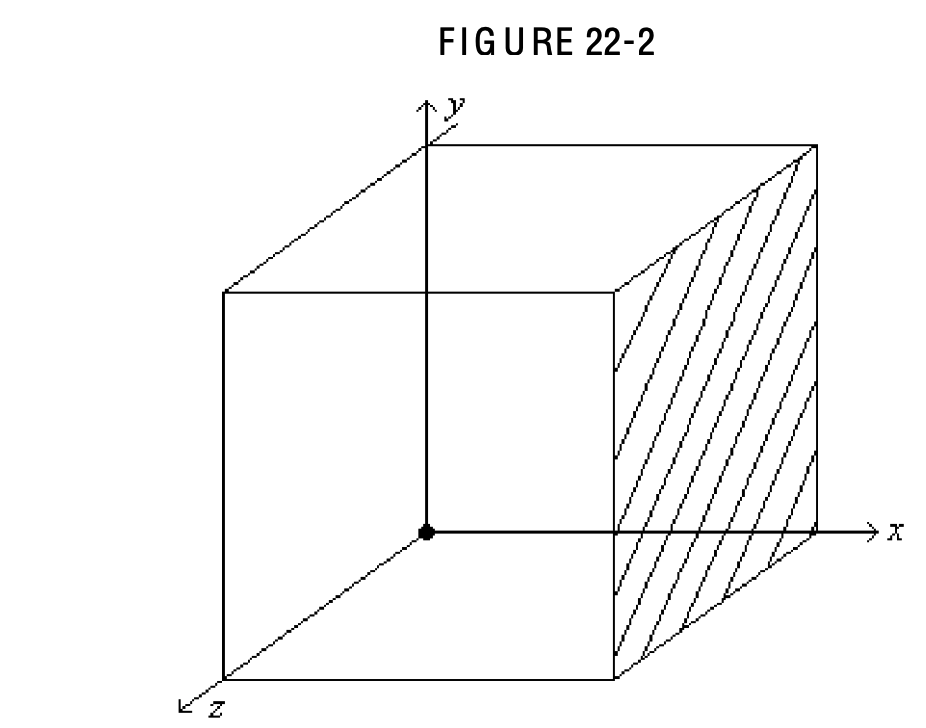
\includegraphics[width=0.3\textwidth]{1.png}\end{center}
  \item[2.] A uniform electric field with a magnitude of \(6\times 10^6 \frac{N}{C}\) is applied to a cube of edge length 0.1 m as shown in Fig. 22-\ 2. If the direction of the E-field is along the +x-axis, what is the electric flux passing through the shaded face of the cube?
  \begin{align*}
    E &= 6\times 10^6\frac{N}{C},~L = 0.1m,\\along&~xaxis,~flux~shaded~side~of~cube\\ \\
    \phi &= E\times A\\
      &= (6\times 10^6\frac{N}{C})\times{(0.1)}^2\\
      &= \boxed{6.0 \times 10^4\frac{N}{C}\cdot{m^2}}\\
  \end{align*}
  \newpage
  \item[3.] A spherical, non-conducting shell of inner radius \(r_1 = 10\) cm and outer radius \(r_2 = 15\) cm carries a total charge Q = 15 \(\mu C\) distributed uniformly throughout its volume. What is the electric field at a distance r = 12 cm from the center of the shell? (SHOW ALL YOUR WORK, DERIVE THE EXPRESSION N)
    \begin{align*}
      \mathcal{V}_{out} &= \frac{4\pi(15^3-10^3)}{3} & \rho = \frac{Q}{\mathcal{V}} &= \frac{15 \times 10^{-6}}{9.9484 \times 10^3}\\
      &= 9948cm^3                                      & &= 1.5078\times 10^{-9} C/cm^3\\
      \mathcal{V}_{in} &= \frac{4\pi(12^3-10^3)}{3} & Q_{in} = \rho\times\mathcal{V}_{in} &=(1.5078\times 10^{-9} C/cm^3)\times(3049cm^3)\\
      &= 3049cm^3                                     & &= 4.59\times 10^{-6}C\\
    \end{align*}
    \begin{align*}
      E &= \frac{kQ_{in}}{r_1}^2\\
        &= \frac{(9\times 10^9 N\cdot m^2/C^2)(4.59\times 10^{-6}C)}{{0.12}^2m}\\
        &= \boxed{2.87 \times 10^6 N/C}\\
    \end{align*}
  \item[4.] A nonconducting spherical shell of inner radius \(R_1\) and outer radius \(R_2\) contains a uniform volume charge density throughout the shell. Use Gauss's law to derive an equation for the magnitude of the electric field at the following radial distances r from the center of the sphere. Your answers should be in terms of \(\rho \), \(R_1\), \(R_2\), r, \(\epsilon_0\) and \(\pi \). (SHOW ALL YOUR WORK, DERIVE THE EXPRESSION N)
  \begin{align*}
    E =& \frac{q}{4\pi\epsilon_0\cdot{r}^2}\\
    a.\ ~r < R_1,~E\cdot 4\pi\cdot{r}^2 =&~\frac{q}{\epsilon_0}\\
    q =&~0\\
    E =&~\boxed{0\frac{N}{C}}\\ \\
    b.\ ~R_1 < r < R_2,~E\cdot 4\pi\cdot{r}^2 =&~\frac{\rho(\frac{4}{3}\pi{r}^3-\frac{4}{3}\pi{R_1}^3)}{\epsilon_0}\\
    E =&~\frac{\rho(r^3-{R_1}^3)}{3\epsilon_0\cdot{r}}\\
    =&~\boxed{\frac{\rho}{3\epsilon_0}\cdot(r-\frac{{R_1}^3}{r^2})}\\ \\
    c.\ ~r > R_2,~E\cdot 4\pi\cdot{r}^2 =&~\frac{\rho(\frac{4}{3}\pi{R_2}^3-\frac{4}{3}\pi{R_1}^3)}{\epsilon_0}\\
    E =&~\boxed{\frac{\rho({R_2}^3-{R_1}^3)}{3\epsilon_0\cdot{r}^2}}
  \end{align*}
  \newpage
  \item[5.] A nonuniform electric field is directed along the x-axis at all points in space. This magnitude of the field varies with x, but not with respect to y or z. The axis of a cylindrical surface, 0.80 m long and 0.20 m in diameter, is aligned parallel to the x-axis, as shown in the figure. The electric fields \(E_1\) and \(E_2\), at the ends of the cylindrical surface, have magnitudes of 9000 \(\frac{N}{C}\) and 5000 \(\frac{N}{C}\) respectively, and are directed as shown. (\(\epsilon_0 = 8.85 \times 10^{-12} \frac{C^2}{N}\cdot m^2\)) The charge enclosed by the cylindrical surface is closest to 
  \item[] \begin{center}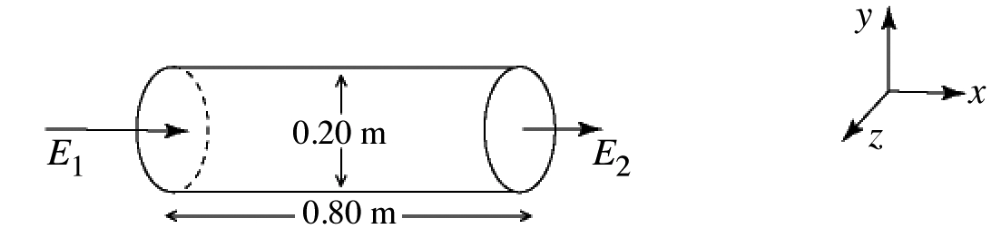
\includegraphics[width=0.4\textwidth]{2.png}\end{center}
  \begin{align*}
    D = 0.2m,~r =&~0.1m,~cross~section=\pi\cdot{(0.1)}^2\\
    \phi_1 =&~\overrightarrow{E_1}\cdot\overrightarrow{A_1},~\phi_2 = \overrightarrow{E_2}\cdot\overrightarrow{A_2}\\
    \phi_1 =&~9000\times\pi\times{10}^{-2}\\
           =&~282.74\frac{N}{C}\cdot{m^2}\\
    \phi_2 =&~5000\times\pi\times{10}^{-2}\\
           =&~157.08\frac{N}{C}\cdot{m^2}\\
    \phi_{net} =&~\phi_2-\phi_1\\
           =&~157.08 - 282.75\\
           =&~-125.67\\ 
           \cong&~\boxed{-1.1nC}
  \end{align*}  
\end{enumerate}
\end{document}